% !TEX root = main.tex

%\section{Proof of Lemma~\ref{lem:2vass-sandwich}: \dvass are \sandwich}\label{sec:sandwich}

\begin{appendixproof}[Proof of Lemma~\ref{lem:2vass-sandwich}]
We extend the definition of nondecreasing functions to many-argument ones:
a function $f: \N^k \to \N$ is \emph{nondecreasing} if it is monotonic
in every argument and $f(n_1, \ldots, n_k) \geq n_1 + \ldots + n_k$.
In the sequel we often bound certain quantities polynomially, but an exact polynomial is irrelevant. 
We thus say that a value $n$ is \emph{polynomially bounded} in $n_1, \ldots, n_k$
if there exists a nondecreasing polynomial $P: \N^k \to \N$ such that $n \leq P(n_1, \ldots, n_k)$
for all $n_1, \ldots, n_k \in \N$. 
We also write $n \leq \poly(n_1, \ldots, n_k)$.

\para{Linear path schemes}
A $d$-dimensional \emph{linear path scheme} ($d$-\LPS in short, or \LPS if dimension is irrelevant) 
is a sequential \vass where every component is either trivial (a singleton) or a simple cycle,
i.e., a \vass whose control graph is a simple path with disjoint simple cycles attached to some states of the path.
We write down \LPS in the following form 
\[
%\Lambda \ = \ 
\alpha_0\beta_1^* \alpha_1 \cdots \alpha_{k-1} \beta_{k}^* \alpha_k,
\]
where each $\alpha_i$ and $\beta_i$ is  a fixed sequence of transitions. 
Thus the cycles $\beta_i$ of an \lps may be repeated arbitrarily many times (possibly zero). 
An \LPS is \emph{simple} (\SLPS) when all $\beta_i$ are single transitions, i.e.,
each component is either trivial or a single self-loop transition.
When considering the reachability relation in a $d$-\LPS, we often implicitly take the first and the last state
of the \LPS as the source and target state, respectively, and consider the reachability $w\tran w'$ between
vectors $w,w'\in\N^d$ only.
% for two vectors $s, t \in \N^d$, denoted $s \trans{\Lambda} t$, instead of reachability from one configuration to another. This is just a shortening of notation meaning that we consider reachability from $p(s)$ to $q(t)$ where $p$ is the first state of $\Lambda$ (before $\alpha_1)$ and $q$ is the last state (after $\alpha_n$) of $\Lambda$.

%\begin{lemma}\label{lem:two-slps}
%There is a nondecreasing polynomial $P$ such that for every \dvass $V$ together with its two states $p$ and $q$,
%such that $\size(V) = M$ there is a finite set $\Gamma$ of \dslps, each of size at most $P(M)$,
%such $p(u) \tran q(v)$ in $V$ if and only if $u \trans{\Lambda} v$ for some \dslps $\Lambda \in \Gamma$.
%\end{lemma}

%\wojtek{Maybe remove Lemma~\ref{lem:two-slps} and move its proof directly to the proof of Lemma~\ref{lem:2vass-sandwich}.}

\begin{lemma}\label{lem:two-slps}
For every \dvass $V$ and two its states $q$, $q'$,
there is a finite set $\Gamma$ of \dslps of size polynomially bounded in $\size(V)$,
such that for all $w,w'\in\N^2$,
\begin{align*} %\label{eq:slps}
 \ \ q(w) \tran q'(w') \text{ in } V \ \iff \ w \tran w' \text{ in some  \dslps in } \Gamma.
\end{align*}
\end{lemma}

\begin{proof}
The claim follows by combination of
Theorem 3.1 from~\cite{DBLP:journals/jacm/BlondinEFGHLMT21}, due to which we get
a finite set $\Gamma$ of \dlps of size polynomially bounded in $\size(V)$ that satisfies the claim,
with Lemma 5.2 from~\cite{DBLP:journals/jacm/BlondinEFGHLMT21} 
(or Theorem 15 from~\cite{DBLP:conf/lics/EnglertLT16}), due to which
we can transform every \dlps $\lambda$ into an \dslps of size polynomially bounded in $\size(\Lambda)$.
%We get that the size of the obtained \dslps are polynomially bounded in the size of the input \dlps.
%Therefore, the resulting \dslps have size at most polynomial also wrt. the size of the considered \dvass, as required.
%Finally, notice that one can upper-bound any polynomial by a nondecreasing polynomial.
%Indeed, it is sufficient to take absolute values of the coefficients, and possibly add the $P(x) = x$, if the starting polynomial is a constant.
\end{proof}

%Here is the previous formulation of the main sandwich lemma, probably not useful  now.
%
%\begin{lemma}\label{lem:two-sandwich}
%There exists a polynomial $R$ such that for any $2$-VASS of size $M$,
%any configuration $s$, any state $q$ and any numbers $N, K, N_t \in \N$
%the set $\reach_q(s)$ is a finite union of:
%\begin{itemize}
%  \item linear sets $a_i + Q_i^* \subseteq \N^2$ such that $\norm(a_i) \leq B_\bg$, $\norm(Q_i) \leq R(M)$, and
%  \item sandwich sets $S_i \subseteq \N^2$ such that there are $b_i \in \N^2$, $P_i \subseteq_{\fin} \N^2$ with $\norm(b_i) \leq B_\sml$,
%  $\norm(P_i) \leq R(M)$ and $b_i + P_i^{\leq B_\bg} \subseteq S_i \subseteq b_i + P_i^*$,
%\end{itemize}
%where $N_s = \norm(s)$, $B_\sml = (N_s + N_t) \cdot (2N \cdot R(M))^K$ and $B_\bg = (N_s + N_t) \cdot (2 N \cdot R(M))^{2K}$. 
%\end{lemma}
%
%\vskip 5cm

%The following lemma, together with Lemma \ref{lem:two-slps}, immediately imply Lemma~\ref{lem:2vass-sandwich}:

%\begin{lemma}\label{lem:slps-sandwich}
%There exists a polynomial $R$ such that for any $2$-SLPS with of norm $N$ and with $n$ states,
%and any vector $s \in \N^2$ with $N_s = \norm(s)$ and any numbers $K, N_t, N_R \in \N$
%the set $\reach(s)$ is a finite union of:
%\begin{itemize}
%  \item linear sets $a_i + Q_i^* \subseteq \N^2$ such that $\norm(a_i) \leq 2R(N) \cdot B_\bg$, $\norm(Q_i) \leq R(N)$, and
%  \item sandwich sets $S_i \subseteq \N^2$ such that there are $b_i \in \N^2$, $P_i \subseteq_{\fin} \N^2$ with $\norm(b_i) \leq B_\sml$,
%  $\norm(P_i) \leq R(N)$ and $b_i + P_i^{\leq B_\bg} \subseteq S_i \subseteq b_i + P_i^*$,
%\end{itemize}
%where
%%$B_\sml = (N_s + N_t + nN) \cdot (2 N_R \cdot R(N))^K$ and $B_\bg = (N_s + N_t + nN) \cdot (2 N_R \cdot R(N))^{4K}$. 
%$B_\sml = (N_s + N_t + n \cdot R(N))$ and $B_\bg = (N_s + N_t + nN) \cdot (2 (N_R + R(N)))^{K+1}$. 
%\end{lemma}

%\begin{lemma}\label{lem:slps-sandwich}
%There exists a polynomial $Q$ such that for every $2$-SLPS $\Lambda$,
%any vector $s \in \N^2$ such that $M = \max(\size(\Lambda), \norm(s))$ and any number $B \in \N$
%the set $\reach(s)$ is a finite union of:
%\begin{itemize}
%  \item linear sets $a_i + Q_i^* \subseteq \N^2$ such that $\norm(a_i) \leq B \cdot Q(M)$, $\norm(Q_i) \leq Q(M)$, and
%  \item sandwich sets $S_i \subseteq \N^2$ such that there are $b_i \in \N^2$, $P_i \subseteq_{\fin} \N^2$ with $\norm(b_i) \leq Q(M)$,
%  $\norm(P_i) \leq Q(M)$ and $b_i + P_i^{\leq B} \subseteq S_i \subseteq b_i + P_i^*$.
%\end{itemize}
%\end{lemma}

\begin{lemma}\label{lem:slps-sandwich}
\dslps are \sandwich.
\end{lemma}

Before proving Lemma~\ref{lem:slps-sandwich}, we use it together with Lemma~\ref{lem:two-slps}
to prove Lemma~\ref{lem:2vass-sandwich}.
%
To this aim consider a \dvass $(V, s)$ where $s=p(w)$, and its state $q$, and let $M=\size(V,s)$.
%$M = \max(\size(V), \norm(s))$.
By Lemma~\ref{lem:two-slps} we get a finite set $\Gamma$ of \dslps such that:
\[
\reach_q(V,s) \ = \ \bigcup_{\Lambda \in \Gamma} \reach(\Lambda, w).
\]
Moreover, for some nondecreasing polynomial $F$, every $\Lambda \in \Gamma$ satisfies
$\size(\Lambda) \leq F(M)$.
By Lemma~\ref{lem:slps-sandwich}, there is a nondecreasing polynomial $G$
such that for every $\Lambda \in \Gamma$ and $B\in\N$, 
the set $\reach(\Lambda,w)$
is 
\kanapka {$G(\size(\Lambda,w))$} {$B$}.
Combining the last two statements, we deduce that $\reach_q(V, s)$ is
\kanapka {$G(F(M))$} {$B$} for every $B\in\N$, as required.
%
Lemma~\ref{lem:2vass-sandwich} is thus proved (once we prove
Lemma~\ref{lem:slps-sandwich}).
\end{appendixproof}

\begin{appendixproof}[Proof of Lemma~\ref{lem:slps-sandwich}]
%
We generalise finite prefixes $P^{\leq B}$ of $P^*$ as follows.
Let $P = \set{p_1, \ldots, p_m}$. 
For a positive vector $c \in (\Npos)^m$ and $T \in \N$ we define
\[
P^{x \cdot c \leq T} := \setof{\Sigma_{i=1}^m n_i \cdot p_i}{\Sigma_{i=1}^m n_i \cdot c_i \leq T}.
\]
In particular, $P^{\leq T} = P^{x\cdot \vec 1  \leq T}$.
In the sequel, sets of the form
\begin{align} \label{eq:hybrid}
a + P^{x \cdot c \leq T} + Q^*,
\end{align}
for $a\in\N^2$, $c \in (\Npos)^{\card P}$ and $P,Q\subseteqfin \N^2$, 
we call \emph{hybrid} sets.

%\begin{lemma}\label{lem:sandwich-raw}
%There exists a nondecreasing polynomial $R$ such that for every $2$-SLPS $\Lambda$,
%any vector $s \in \N^2$ and $M = \max(\size(\Lambda), \norm(s))$ the set of vectors reachable by $\Lambda$ from $s$ is a finite union of sets $S$ of the following form.
%For each $S$ there exists a base vector $b \in \N^2$, sets of periods vectors $P, Q \subseteq_\fin \N^2$, vector $c \in \N^{|P|}$ and threshold $T \in \N$
%such that
%\[
%S = b + P^{c \cdot x \leq T} + Q^*,
%\]
%where $\norm(b), \norm(P \cup Q), \norm(c) \leq R(M)$ and $c_i \geq 1$ for each $i \in [1, |P|]$.
%\end{lemma}

\begin{lemma}\label{lem:sandwich-raw}
For every \dslps $(\Lambda,s)$,
% any vector $s \in \N^2$ and $M = \size(\Lambda, s)$
the set $\reach(\Lambda,s)$ is a finite union of hybrid sets \eqref{eq:hybrid}, 
% of vectors reachable by $\Lambda$ from $s$ is a finite union of sets $S$ of the following form.
%For each $S$ there exists a base vector $b \in \N^2$, sets of periods vectors $P, Q \subseteq_\fin \N^2$, vector $c \in \N^{|P|}$ and threshold $T \in \N$ such that
%\[
%S = b + P^{c \cdot x \leq T} + Q^*,
%\]
where $\norm(a),  \norm(c), \norm(P \cup Q)$ are bounded polynomially in $\size(\Lambda,s)$.
% and $c_i \geq 1$ for each $i \in [1, |P|]$.
\end{lemma}

Before proving Lemma~\ref{lem:sandwich-raw} we use it to prove Lemma~\ref{lem:slps-sandwich}.
We need to argue that there is a nondecreasing polynomial $F$ such that 
for every \dslps $(\Lambda, s)$ and $B\in\N$, the set $\reach(\Lambda,s)$ is
\kanapka {$F(M)$} {$B$}, where $M=\size(\Lambda,s)$.
%
%Recall that according to the definition of polynomial approximability
%we need to prove that for each $B \in \N$ there is a polynomial $F$ such that for $M = \size(\Lambda, s)$
%the set of points reachable from $s$ via $\Lambda$ is a finite union of:
%\begin{itemize}
%  \item linear sets $S = a + Q^* \subseteq \N^2$ such that $\norm(a) \leq B \cdot F(M)$, $\norm(Q) \leq F(M)$, and
%  \item $B$-approximations of linear sets, namely $S \subseteq \N^2$ such that there are $a \in \N^2$, $Q \subseteq_{\fin} \N^2$ with $\norm(a), \norm(Q) \leq F(M)$, and $a + Q^{\leq B} \subseteq S \subseteq a + Q^*$.
%\end{itemize}
%By Lemma~\ref{lem:sandwich-raw} we have that the considered set is a finite union of sets
%$S$ of the form
%\[
%S = b + P^{c \cdot x \leq T} + Q^*
%\]
%with $\norm(b), \norm(P \cup Q), \norm(c) \leq R(M)$ for some nondecreasing polynomial $R$
%and $c_i \geq 1$ for each $i \in [1, |P|]$.
We fix the nondecreasing polynomial $F(x) = R(x) + R^2(x)$, where $R$ is a polynomial witnessing 
Lemma~\ref{lem:sandwich-raw}, and some arbitrary $B \in \N$,
and prove that each hybrid set $H$ \eqref{eq:hybrid} 
of Lemma~\ref{lem:sandwich-raw} is
\kanapka {$F(M)$} {$B$}.
% 
%It is enough to check each set $S$ separately, namely to check that for each $B \in \N$
%the set $S$ is $(F(M), B)$-approximately semi-linear.
%Fix $B \in \N$.
% and consider the set $b + P^{c \cdot x \leq T} + Q^*$ for some $T \in \N$.
%
We distinguish two cases.
If $T \geq R(M) \cdot B$ then, since $\norm(c)\leq R(M)$, we have
%because each entry of $c$ is at most $R(M)$, we have that
\[
a + (P \cup Q)^{\leq B} \ \subseteq \ H \ \subseteq \ a + (P \cup Q)^*,
\]
and $\norm(a), \norm(P \cup Q) \leq R(M) \leq F(M)$, as required. 
%
On the other hand, if  $T < R(M) \cdot B$ then $H$ is a finite union
of linear sets of the form $u + Q^*$ for $u \in b + P^{c \cdot x \leq T}$, where
\begin{align*}
\norm(u) \ \leq \ \norm(a) + \norm(P) \cdot T 
\ \leq \ R(M) + R(M)^2 \cdot B \leq  F(M) \cdot B,
\end{align*}
as required. 
As before,  $\norm(Q) \leq R(M) \leq F(M)$.
This completes the proof of Lemma~\ref{lem:slps-sandwich} (once
we prove Lemma~\ref{lem:sandwich-raw}). 
\end{appendixproof}
%\begin{align*}
%\norm(u) & \leq \norm(b) + \norm(P) \cdot T \\
%& \leq \norm(s) + n \cdot R(N) + R(N) \cdot B 
%& \leq B + B + R(N) \cdot B = B \cdot (R(N) + 2)  \\
%& \leq B \cdot 2 R'(N)
%\end{align*}
%for $R'(x) = R(x) + 2$. The second to last inequality holds as clearly $\norm(s) \leq B$ and $n \cdot R(N) \leq B$.
%Thus we get Lemma~\ref{lem:slps-sandwich} for the polynomial $R'$.


\begin{appendixproof}[Proof of Lemma~\ref{lem:sandwich-raw}]
The proof occupies the rest of this section.
%The rest of this subsection is devoted to the proof of Lemma~\ref{lem:sandwich-raw}.
We rely on an insightful characterisation of paths of \slps \cite[Theorem 4.16]{DBLP:conf/focs/0001CMOSW24},
which we state below using a slightly different terminology.
%We formulate an easy consequence of this theorem here, in a slightly different and simpler phrasing.
%Before we need to define a few notions.
%
Speaking informally, a \emph{detailing} of an \slps 
$\Lambda = \alpha_0 \beta_1^* \alpha_1 \ldots \alpha_{k-1} \beta_k^* \alpha_k$
is any \slps obtained by fixing exponents of some of the cycles of $\Lambda$.
Formally, a detailing of $\Lambda$ is any $\Lambda'$ obtained by choosing a subset $S \in [1,k]$ and,
for all $i \in S$, by replacing the cycle $\beta_i$ by a path $\beta_i^{n_i}$, for some $n_i\in\N$, 
which becomes an infix of the simple path of $\Lambda'$.
The number of cycles of $\Lambda'$ is thus $k-\card{S}$.
%
An \dslps is \emph{zigzagging} if the effect of its every cycle $\beta_i$ 
belongs either to the quadrant $\Npos \times (-\Npos)$,
or to the quadrant $(-\Npos) \times \Npos$, and additionally effects of every two consecutive cycles belong 
to different quadrants
(the effects of cycles $\beta_1, \ldots, \beta_k$ thus alternate between quadrants), and the effect of the first cycle belongs to $\Npos \times (-\Npos)$ and the effect of the last cycle belongs to $(-\Npos) \times \Npos$.
Finally, an \slps is \emph{short} if it contains at most three cycles, $k\leq 3$.
For $B\in\N$,
a path 
\[
s_0 \trans{\alpha_0} t_0 \trans{\sigma_1} s_1 \trans{\alpha_1} t_1 \ \cdots \ s_{k-1} \trans{\alpha_{k-1}} t_{k-1} \trans{\sigma_{k}} s_k \trans{\alpha_k} t_k
\]
of an \dslps,
where $\sigma_i \in\beta^*$ for $i\in\setto k$, is called \emph{$B$-close} if all the vectors $x\in \{s_0, t_0, s_1, t_1, \ldots, s_k, t_k\}$,
called \emph{midpoints} below,
are \emph{$B$-close} to some axis, namely either $x\in \setfromto 0 B \times \N$ or 
$x\in \N\times\setfromto 0 B$.

\begin{theorem}[Thm 4.16 in~\cite{DBLP:conf/focs/0001CMOSW24}]\label{thm:2slps-zigzag}
For every \dslps $\Lambda$ there is $B\leq \poly(\size(\Lambda))$
such that for every path $s \tran t$ in $\Lambda$ 
there is a detailing $\Lambda' = \Lambda_1 \Lambda_2 \Lambda_3$ of $\Lambda$  
of $\size(\Lambda')\leq \poly(\size(\Lambda))$ and $u, u' \in \setfromto 0 B \times \N$ such that
\begin{enumerate}
%  \item $\size(\Lambda') \leq \poly(M)$,
 %$P(\size(\Lambda))$,
  \item $\Lambda_1$ and $\Lambda_3$ are short, 
  \item $\Lambda_2$ is zigzagging,
  \item there are paths $s \tran u$ in $\Lambda_1$, 
  a $B$-close path $u \tran u'$ in $\Lambda_2$, and 
  $u'\tran t$ in $\Lambda_3$.
\end{enumerate}
%For any $2$-SLPS $\Lambda$, vectors $s, t \in \N^2$ such that $s \trans{\Lambda} t$ and $M = \max(\norm(s), \size(\Lambda))$
%there exists a bound $B = \poly(M)$ and a detailing $\Lambda'$ of $\Lambda$ such that $\Lambda' = \Lambda_1 \Lambda_2 \Lambda_3$
%with the following properties
%\begin{itemize}
%  \item $\size(\Lambda') \leq \poly(M)$,
% %$P(\size(\Lambda))$,
%  \item $\Lambda_1$ and $\Lambda_3$ are short, while $\Lambda_2$ is zigzagging
%  \item there are $u_1, u_2 \in [0,B] \times \N$ such that $s \trans{\Lambda_1} u_1 \trans{\pi} u_2 \trans{\Lambda_3} t$
%  for some $B$-close $\Lambda_2$-path $\pi$.
%\end{itemize}
\end{theorem}

%Due to Theorem~\ref{thm:2slps-zigzag}, in the proof of 
%Lemma~\ref{lem:sandwich-raw} we may safely restrict to paths of the above form. 
Fix in the sequel $B$ given by Theorem~\ref{thm:2slps-zigzag}.
There are only finitely many detailings $\Lambda'$ of $\Lambda$ of a bounded size,
only finitely many possible decompositions of $\Lambda'$ into $\Lambda_1$, $\Lambda_2$ and $\Lambda_3$,
and only finitely many values of $u_1, u'_1\in\setfromto 0 B$.
By Theorem~\ref{thm:2slps-zigzag}, vectors $t$ reachable from $s$ in $\Lambda$ are exactly those
reachable from $s$ in some of detailing $\Lambda'$.
Therefore it is enough
to show Lemma~\ref{lem:sandwich-raw} for the set of vectors $t\in\N^2$ reachable by paths as in point 3 above,
in a fixed \slps $(\Lambda',s)$, where $\Lambda' = \Lambda_1 \Lambda_2 \Lambda_3$ satisfies points 1, 2 above,
and where $u_1 = b$ and $u'_1 = b'$ for some fixed $b,b'\in\setfromto 0 B$.

In a path $u\tran u'$, every second midpoint is $B$-close to one axis,
say $x\in \setfromto 0 B \times \N$,
while the remaining midpoints are $B$-close to the other one.
We relax this requirement slightly, by dropping the latter condition.
A path $u \tran u'$  in the zigzagging \slps $\Lambda_2$
is \emph{$B$-vertical-close} if $u$, $u'$ and every second midpoint $x$
are $B$-close to the vertical axis, namely $x \in \setfromto 0 B \times \N$
(thus the remaining endpoints on the path do not have to be $B$-close to the horizontal axis).
In order to have more flexibility in the proof of Lemma~\ref{lem:sandwich-raw},
in the sequel we consider those paths in $\Lambda'$, as in point 3 in Theorem~\ref{thm:2slps-zigzag}, where the infix
$u\tran u'$ is $B$-vertical-close but not necessarily $B$-close.
Notice that by relaxing the condition to $B$-vertical-closeness
we enlarge the set of considered paths, but do not enlarge the set of reachable points,
as every $t$ such that $s \tran t$ is already reachable by the paths with the middle path being even $B$-close.
We denote by $\reach(\Lambda', s)$ the set of all vectors $t\in\N^2$ reachable by such a path $s\tran t$ with
the middle part being $B$-vertical-close.

We formulate below Claims \ref{cl:prefix}, \ref{cl:infix} and \ref{cl:suffix}
(taking care of a prefix, infix, and suffix, respectively, of a path $s\tran t$), 
show how they imply Lemma~\ref{lem:sandwich-raw}, and finally proceed with the proofs of the three claims.
To this aim we introduce some more notation.
Given a start $a \in \N$, a difference $r \in \N$, and a bound $T \in \N_\infty = \N\cup\{\infty\}$,
the set $a + \{r\}^{\leq T}$ is called \emph{$(a, r, T)$-arithmetic}. 
We omit brackets and write $a + r^{\leq T}$.
In particular, $a + r^{\leq 0} = \{a\}$.
%The first claim essentially says that it is enough to consider only a finite number
%of arithmetic sequences for vectors reachable from $s$ by a short $2$-SLPS.
A \dslps  $\alpha_1 \beta_1^* \alpha_2 \beta_2^*$ is \emph{one-turn} if 
$\eff(\beta_1) \in \Npos  \times -\Npos$ and $\eff(\beta_2) \in -\Npos  \times \Npos$
(it is thus a special case of short zigzagging \dslps).
%
For a set $S\subseteq \N^2$, we use the notation $\reach(\Lambda, S) = \bigcup_{s\in S} \reach(\Lambda, s)$.

In Claims \ref{cl:prefix}, \ref{cl:infix} and \ref{cl:suffix}, we focus on source/target vectors
in $\setfromto 0 B \times \N$ and, intuitively speaking, on arithmetic subsets of each 'line' $\{b\}\times \N$.
First, Claim \ref{cl:prefix} states that the reachability set of a short \dslps, intersected with each line,
is a finite union of arithmetic sets.
Second, Claim \ref{cl:infix} states that the reachability set of a one-turn \dslps from 
an arithmetic set inside a line, intersected with another line, is a finite union of arithmetic sets.
Importantly, the starting point grows only additively, by a polynomially bounded amount, 
as we will apply Claim \ref{cl:infix} $\OO(k)$ times.
Finally, Claim \ref{cl:suffix} states that the reachability set of a short \dslps, from an arithmetic set
inside a line, is a finite union of hybrid sets.
All quantities in the claims are bounded polynomially.

\begin{claim}\label{cl:prefix}
For every short \dslps $(\Lambda,s)$ 
%$M = \size(\Lambda, s)$  
and $u_1 \in [0,B]$,
the set $\{u_2 \mid (u_1, u_2) \in \reach(\Lambda,s)\}$ is a finite union of $(a, r, T)$-arithmetic sets, where
$a \leq \poly(B,M)$, $r \leq \poly(M)$, and $M=\size(\Lambda,s)$.
\end{claim}
%
\begin{claim}\label{cl:infix}
Let $\Lambda$ be a one-turn \dslps,
and $S_1 = a + r^{\leq K}$ for some $a, r, K \in \N$.
Let $u_1, v_1 \in [0, B]$.
The set $R(S_1) := \{v_2 \mid \exists_{u_2 \in S_1} (u_1, u_2) \tran (v_1, v_2) \text{ in } \Lambda\}$
is a finite union of $(a', r', T')$-arithmetic sets with
$a' \leq a + \poly(B,M,r)$ and $r' \leq \max(\poly(M),r)$, where $M=\size(\Lambda)$.
\end{claim}

%
%The last claim takes care about the short suffix of the $2$-SLPS.
%
%\begin{claim}\label{cl:suffix}
%There is a polynomial $R$ such that for every short $2$-SLPS $\Lambda$ such that $M=\size(\Lambda)$, $S_1 = b_1 + \set{p_1}^{\leq T}$
%and $N = \norm(p_1)$ the set $S_2 = \reach_{\Lambda}(S_1)$
%is a finite union of sets $b_2 + P_2^{a \cdot x \leq T} + Q_2^*$ for $\norm(P_2 \cup Q_2), \norm(a) \leq R(N) \cdot R(M)$, $\norm(b_2) \leq (\norm(b_1)+1) \cdot R(N) \cdot R(M)$ and additionally $a_i \geq 1$ for each $i$. 
%\end{claim}
%
\begin{claim}\label{cl:suffix}
For every short \dslps $\Lambda$ and $u= (u_1, u_2), p = (p_1, p_2)\in\N^2$, 
the set $\reach(\Lambda, u + \set{p}^{\leq T})$
is a finite union of hybrid sets \eqref{eq:hybrid},
where $\norm(a), \norm(c), \norm(P), \norm(Q) \leq \poly(\size(\Lambda), \norm(u),\norm(p))$.
\end{claim}

We use the three  claims to derive Lemma~\ref{lem:sandwich-raw}.
As said above,
we consider a fixed \slps $\Lambda' = \Lambda_1 \Lambda_2 \Lambda_3$ and source $s\in\N^2$,
and focus on the set $\reach(\Lambda', s)$ of vectors $t\in\N^2$ such that
there are paths 
%
\begin{align} \label{eq:paths}
\text{$s \tran u$ in $\Lambda_1$,  \ \  
a $B$-vertically close path $u \tran u'$ in $\Lambda_2$, \ \ 
and   $u'\tran t$ in $\Lambda_3$,}
\end{align}
%
for some $u,u'\in \setfromto 0 B \times \N$, where 
$u_1 = b$ and $u'_1 = b'$ are fixed.
Let $M':=\size(\Lambda',s) \leq \poly(M)$.
%
%we aim at characterising the set of vectors $t \in \N^2$ such that
%there is $B \leq \poly(M)$, $u_1, u_2 \in [0, B] \times \N$ and paths $s \trans{\Lambda_1} u_1 \trans{\pi} u_2 \trans{\Lambda_3} t$
%where $\pi$ is a $B$-vertical-close $\Lambda_2$-path. Let us fix some $x_1, x_2 \in [0,B]$ such that $u_1[1] = x_1$ and $u_2[1] = x_2$.
%
%Recall that $M = \size(\Lambda, s)$ and by Theorem~\ref{thm:2slps-zigzag} we have that $\size(\Lambda') \leq \poly(M)$.
First, by Claim~\ref{cl:prefix}, the set
$\{u_2 \mid (u_1, u_2) \in \reach(\Lambda_1,s)\}$ is a finite union of $(a, r, T)$-arithmetic sets,
where $a, r$ are bounded polynomially in $M'$ and $B$.
%
Second,
a path $u\tran u'$ is a concatenation of $\ell\leq \size(\Lambda_2) \leq \poly(M')$
paths of one-turn \slps. 
By $\ell$-fold application of Claim~\ref{cl:infix}, the set
$\{u'_2 \mid (u'_1, u'_2) \in \reach(\Lambda_1 \Lambda_2,s)\}$
is a finite union of arithmetic sets
$a' + (r')^{\leq T'}$, where
%\begin{equation}\label{eq:rprim}
$a', r' \leq \poly(\size(\Lambda_2)) \leq \poly(M')$.
%\end{equation}
Indeed, the bound on $a'$ comes from $\ell$-fold addition of values bounded by 
$\poly(B, \poly(M'), r)\leq \poly(B, \poly(M'), \poly(M'))$,
itself bounded by $\poly(M')$:
%
\begin{equation}\label{eq:aprim}
a' \leq a + \ell \cdot \poly(M') \leq a + \poly(M') \leq \poly(M').
\end{equation}
%
Finally, by Claim~\ref{cl:suffix} the set $\reach(\Lambda',s)$ is a finite union of hybrid sets \eqref{eq:hybrid},
where
$
\norm(a)$, $\norm(c)$, $\norm(P \cup Q) \leq \poly(M', B) \leq \poly(M).
$ 
%By equations~\eqref{eq:rprim}~and~\eqref{eq:aprim} we have $N = \max(a', r') \leq \poly(M)$.
%Therefore
%\[
%\norm(c), \norm(b), \norm(P \cup Q) \leq \poly(M),
%\]
We conclude the proof of Lemma~\ref{lem:sandwich-raw}, keeping in mind that
it still remains to demonstrate Claims~\ref{cl:prefix},~\ref{cl:infix},~and~\ref{cl:suffix}.

\medskip

Here is  a corollary of Lemma~\ref{lem:taming}, useful in the proofs of the three claims:
%
\begin{lemma}\label{lem:solutions}
Consider a system $A\cdot x = b$ of $m$ Diophantine linear equations with $n$ unknowns,
where absolute values of coefficients are bounded by $N$.
Then, the set of solutions is of a form $U+P^*$, where
$\norm(U \cup P) \leq \poly(nN)^{\poly(n,m)}$.
\end{lemma}

\begin{proof}
The solution set is of the form $U+P^*$,
where $U$ is the set of pointwise minimal nonnegative integer solutions of the system,
and $P$ is the set of pointwise minimal nonnegative integer solutions of its homogeneous version
$A\cdot x = \vec 0$.
By Lemma~\ref{lem:taming} each element of $U \cup P$ has norm at most $M= \Oo(nN)^m$.
Therefore, the number of different solutions is at most $(M+1)^n$, which implies 
$\norm(U \cup P) \leq \poly(nN)^{\poly(n,m)}$.
\end{proof}
%
In the sequel we apply Lemma~\ref{lem:solutions} in case when $n$ and $m$ are constants,
in which case Lemma \ref{lem:solutions} yields the bound $\norm(U+P) \leq \poly(N)$.

\begin{proof}[Proof of Claim~\ref{cl:prefix}]
For $d \in \setto 2$ and
a path $\gamma$, let $\eff_j(\gamma)$ denote the $j$-th coordinate of $\eff(\gamma)$, and
let $\drop_j(\gamma)\in\N$ be the maximal value of $-\eff_j(\delta)$, where $\delta$ ranges over prefixes of $\gamma$,
that is  the maximal amount by which the $j$-th coordinate can be decreased along $\gamma$.

\Wlog we assume that $\Lambda$ has exactly three loops, 
$\Lambda = \alpha_1\beta_1^{*}\alpha_2\beta_2^{*}\alpha_3\beta_3^{*}\alpha_4$. 
We describe paths $s = (s_1, s_2) \tran (u_1, u_2)$ in $\Lambda$,
\begin{align*}
(s_1, s_2) = \ & 
(a^1_1, a^1_2) \trans{\alpha_1} (b^1_1, b^1_2) \trans{\beta_1^{n_1}}
(a^2_1, a^2_2) \trans{\alpha_2} (b^2_1, b^2_2) \trans{\beta_2^{n_2}} \\
& (a^3_1, a^3_2) \trans{\alpha_3} (b^3_1, b^3_2) \trans{\beta_3^{n_3}}
(a^4_1, a^4_2) \trans{\alpha_4} (b^4_1, b^4_2) = (u_1, u_2),
\end{align*}
by the following system of linear Diophantine inequalities, with unknowns 
$a^{i}_1, a^{i}_2, b^{i}_1, b^{i}_2$, for $i\in\setto 4$, and $n_i$, for $i\in\setto 3$,
ensuring that the effects of $\alpha_i$ and $\beta_i^{n_i}$ are respected, 
and that all points along $\alpha_i$ remain nonnegative 
:
%
%\begin{itemize} 
%\item $a^{i}_1, a^{i}_2$, for $i\in\setto 4$, denoting the midpoint just before the execution of $\alpha_{i}$ 
%(for $i=1$, the source);
%\item $b^{i}_1, b^{i}_2$, for $i\in\setto 4$, denoting the midpoint just after  the execution of $\alpha_{i}$
%(for $i=4$, the target);
%\item $n_i$, for $i\in\setto 3$, denoting the number of times $\beta_i$ is executed.
%\end{itemize}
%
%\noindent
%Therefore the path from $s$ to $t$ has the following form:
%
%The following system of inequalities $\U$ guarantees that the path of $\Lambda$ is inside the positive quadrant.
%
\begin{align*}
a^{i}_j + \eff_j(\alpha_i) \ = \ & \ b^{i}_j  & a^1_j \ = \ & \ s_j \\
b^{i}_j + n_i \cdot \eff_j(\beta_i) \ = \ & \ a^{i+1}_j & b^4_1 \ = \ & \ u_1 \\
a^i_j - \drop_j(\alpha_i) \ \geq \ & \ 0 
\end{align*}
%
Notice that each $\beta_i$ is a single transition, so nonnegativity of $(b_i^1, b_i^2)$ and $(a_{i+1}^1, a_{i+1}^2)$
implies that all the vectors along  $\beta_i^{n_i}$ are also nonnegative. Therefore, we do not need to
add an analog of $a^i_j - \drop_j(\alpha_i) \geq 0$ for $\beta_i$ to the above system.
%
%\begin{enumerate}[(1)]
%\item For each $i \in [1,4]$ and $d \in [1,2]$ we take care of the effect of $\alpha_i$:\label{eq:LPS_eff_1}
%$$a_{i}^d + \eff_d(\alpha_i) = b_{i}^d$$
%\item For each $i \in [1,3]$ and $d \in [1,2]$ we take care of the effect of $\beta_i$:\label{eq:LPS_eff_2}
%$$b_{i}^d + n_i \cdot \eff_d(\beta_i) = a_{i+1}^d$$
%\item For each $i \in [1,4]$ and $d \in [1,2]$ we take care that counter remains nonnegative along $\alpha_i$
%$$a_i^d + \drop_d(\alpha_i) \geq 0$$ \label{eq:LPS_non}
%\item For each $d \in [1,2]$ we take care that a path starts in $s$.
%$$a_1^d = s_d$$\label{eq:LPS_start}
%\item We take care that the first coordinate of the target is equal to $x$.
%$$b_4^1 = x$$\label{eq:LPS_end}
%\end{enumerate}
%Notice that . 
By adding dummy variables we change inequalities into equations,
thus obtaining a system $\U$ of linear Diophantine equations.
All the coefficients in $\U$ are bounded by $\max(B, M)$, 
and all coefficients in its homogeneous version are bounded by $M$.
Therefore, by Lemma~\ref{lem:solutions} the solution set of $\U$ is $U+P^*$,
where $\norm(U) \leq \poly(B,M)$ and $\norm(P) \leq \poly(M)$.
By projecting the solution set to the variable $b^4_2$, we deduce that
the set $S:=\{u_2 \mid (u_1, u_2) \in \reach(\Lambda,s)\}$ is a finite union of 
linear sets $a+X^*$, where $a \leq P_1(B,M)$ and $X \subseteq [0,P_2(M)]$,
for some nondecreasing polynomials $P_1, P_2$.
%
% $a \leq \poly(B,M)$ and $X \subseteqfin \N$, such that
%for each $x \in X$ we have $x \leq \poly(M)$.
%
%$(a, r, T)$-arithmetic sets, where
%$a \leq \poly(B,M)$, $r \leq \poly(M)$, and $M=\size(\Lambda,s)$.
%
\begin{claim}\label{cl:linear-1dim}
For every $a,b \in \N$ and $B \subseteq [1,b]$, the linear set $a+B^*$ is a finite union
of arithmetic sets $c + d^*$, where $c \leq a+b^3$ and $d \leq b$.
\end{claim}
\begin{proof}
Let $B = \set{b_1, \ldots, b_m}$.
Let $n \in a + B^*$, and let $(k_1, \ldots, k_m) \in \N^m$ be the lexicographically smallest vector such that
$n = a + \sum_{i=1}^m k_i \cdot b_i$.
We observe that $k_i < b$ for all $i\in\setto {m-1}$ since,
% may hold for at most one $i\in\setto m$.
supposing $k_i \geq b$ for
$i < m$, we would get a lexicographically smaller  vector
\[
(k_1, \ldots, k_{i-1}, k_i - b_m, k_{i+1}, \ldots, k_m+ b_i) \in \N^m
\]
with the same property. 
Thus $n \in a + r + b_m^*$,
where $r = \sum_{i<m} k_i \cdot b_i \leq b^3$. 
As $n\in a+ B^*$ was chosen arbitrarily, we deduce
%This means any $n \in a+B^*$ satisfies $n \in c+b_i^*$, where $c \leq a+b^3$. In consequence
\[
a+B^* \ = \bigcup_{c \leq a+b^3, c \in a+B^*} c + b_m^*,
\]
which concludes the proof of Claim~\ref{cl:linear-1dim}.
\end{proof}
%
By Claim~\ref{cl:linear-1dim}, the set $S$ is a finite union of arithmetic sets  $a+x^*$, where 
$a \leq P_1(B,M) + P_2(M)^3$ and $x \leq P_2(M)$,
which concludes the proof of Claim~\ref{cl:prefix}.
Notice that we actually get $T = \infty$ or $T=0$ in all the arithmetic sets, but that is not needed for our considerations.
\end{proof}

% !TEX root = main.tex

\begin{proof}[Proof of Claim~\ref{cl:infix}]
Fix a  one-turn \slps $\Lambda=\alpha_1\beta_1^*\alpha_2\beta_2^*$, and
let $M:=\size(\Lambda)$ and $S_2 := R(S_1)$.
Our goal is to show that the set $S_2 = \bigcup_{c\in S_1} R(\{c\})$
%For $c \in S_1$ let us denote $R(c) = \set{v_2 \in (u_1, c) \tran (v_1, v_2)}$.
%Let $R(S_1) = \bigcup_{c \in S_1} R(c)$. Our goal is to show that $R(S_1)$ 
is a finite union
of $(a', r', T')$-arithmetic sequences for $a' \leq a + \poly(B, M, r)$ and $r' \leq \poly(M)$.
We write $R(c)$ instead of $R(\{c\})$.

Let $\eff(\beta_1) = (x_1, -y_1)$ and $\eff(\beta_2) = (-x_2, y_2)$, for some $x_1, x_2, y_1, y_2 \in \Npos$.
% (recall that $\beta_1$
%and $\beta_2$ belong to the corresponding quadrants by assumptions of Claim~\ref{cl:infix}).
Every path $\rho = \alpha_1\beta_1^{n_1}\alpha_2\beta_2^{n_2}$ is determined by 
a pair $(n_1,n_2) \in \N^2$,
and hence when $(u_1, u_2) \tran (v_1, v_2)$, we may also write $(u_1, u_2) \trans {(n_1,n_2)} (v_1, v_2)$
for $(n_1, n_2)\in\N^2$, or 
$(u_1, u_2) \trans {(n_1,n_2)}$ when the target vector is not relevant.
%and we say that $\rho = \rho(n_1, n_2)$.
Whenever this happens, we necessarily have the equality
%We are interested in possible $c_2 \in \N$ such that there is $c_1 \in S_1$ such that $(b_1, c_1) \trans{(n_1, n_2)} (b_2, c_2)$
%for some $n_1, n_2 \in \N$. Notice that looking at the first coordinate gives the following equation
$
u_1 + \eff_1(\alpha_1 \alpha_2) + n_1 x_1 - n_2 x_2 = v_1
$
of effects on the first coordinate,
which we transform to an equation with two unknowns $n_1,  n_2$:
\begin{equation}\label{eq:xy}
n_1 x_1 - n_2 x_2 = v_1 - u_1 - \eff_1(\alpha_1 \alpha_2).
\end{equation}
%
The set of solutions $(n_1, n_2)$ of~\eqref{eq:xy} is of the form $w+p^*$, 
where $w = (w_1, w_2) \in \N^2$ is the minimal solution of~\eqref{eq:xy}
and $p = (p_1, p_2) \in \N^2$ is the minimal solution of its uniform version, $n_1 x_1 - n_2 x_2 = 0$.
By Lemma~\ref{lem:solutions} we get $\norm(w) \leq \poly(B, M)$. One can easily observe that $\norm(p) \leq 2M$
($(x_1, x_2) = (n_2, n_1)$ is a solution).
%
Let $\eff_2(w) = -w_1 y_1 + w_2 y_2$ and $\eff_2(p) = -p_1 y_1 + p_2 y_2\in \N$ be 
the effects induced by $w$ and $p$, respectively, on the second coordinate.

\begin{example}\label{ex:infix}
\begin{figure}[t]
\vspace{-2cm}
\begin{minipage}{0.5\textwidth}
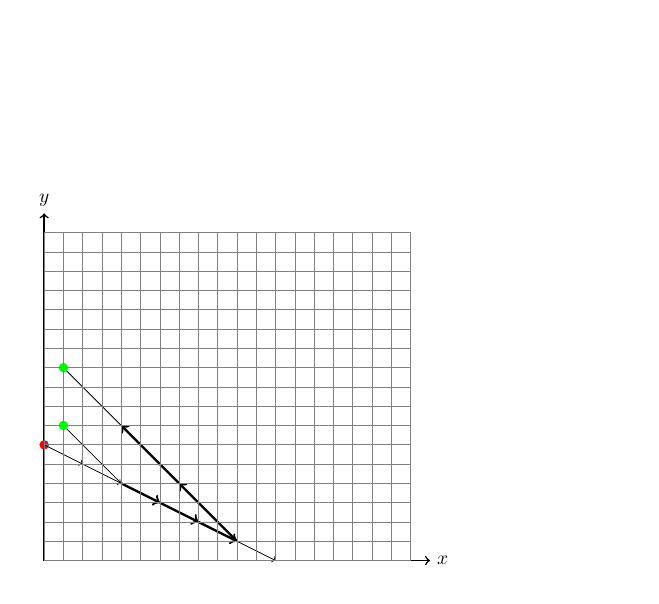
\begin{tikzpicture}[scale=0.35]
\scalebox{0.7}{
\draw[->, thick] (0, 0) -- (20, 0) node[right] {$x$};
\draw[->, thick] (0, 0) -- (0, 18) node[above] {$y$};

\fill[red] (0,6) circle (7pt);

\draw[->] (0,6) -> (2,5);
\draw[->] (2,5) -> (4,4);
\draw[very thick,->] (4,4) -> (6,3);
\draw[very thick,->] (6,3) -> (8,2);
\draw[very thick,->] (8,2) -> (10,1);
\draw[->] (10,1) -> (12,0);

\draw[->] (4,4) -> (1,7);
\fill[green] (1,7) circle (7pt);

\draw[very thick,->] (10,1) -> (7,4);
\draw[very thick,->] (7,4) -> (4,7);
\draw[->] (4,7) -> (1,10);
\fill[green] (1,10) circle (7pt);

\draw[step=1, gray, thin] (0, 0) grid (19, 17);
}
\end{tikzpicture}
\end{minipage}
\begin{minipage}{0.5\textwidth}
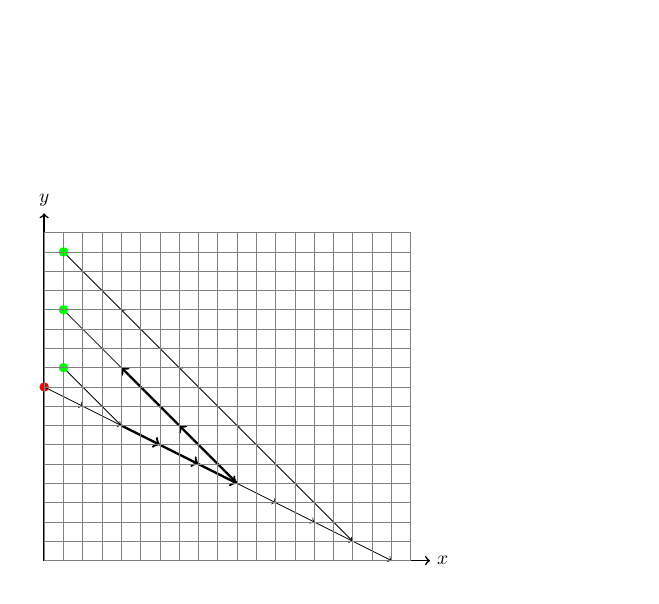
\begin{tikzpicture}[scale=0.35]
\scalebox{0.7}{
\draw[->, thick] (0, 0) -- (20, 0) node[right] {$x$};
\draw[->, thick] (0, 0) -- (0, 18) node[above] {$y$};

\fill[red] (0,9) circle (7pt);

\draw[->] (0,9) -> (2,8);
\draw[->] (2,8) -> (4,7);
\draw[very thick,->] (4,7) -> (6,6);
\draw[very thick,->] (6,6) -> (8,5);
\draw[very thick,->] (8,5) -> (10,4);
\draw[->] (10,4) -> (12,3);
\draw[->] (12,3) -> (14,2);
\draw[->] (14,2) -> (16,1);
\draw[->] (16,1) -> (18,0);

\draw[->] (4,7) -> (1,10);
\fill[green] (1,10) circle (7pt);

\draw[very thick,->] (10,4) -> (7,7);
\draw[very thick,->] (7,7) -> (4,10);
\draw[->] (4,10) -> (1,13);
\fill[green] (1,13) circle (7pt);

\draw[->] (16,1) -> (13,4);
\draw[->] (13,4) -> (10,7);
\draw[->] (10,7) -> (7,10);
\draw[->] (7,10) -> (4,13);
\draw[->] (4,13) -> (1,16);
\fill[green] (1,16) circle (7pt);

\draw[step=1, gray, thin] (0, 0) grid (19, 17);
}
\end{tikzpicture}
\end{minipage}

\caption{Left: $u_2 = 6$, $S_2 = \set{7,10}$. Right: $u_2 = 9$, $S_2 = \set{10,13,16}$.
Thick vectors add up to $p$.}
\label{fig:infix}
\end{figure}

Let $\alpha_1$ and $\alpha_2$ be empty sequences, $\eff(\beta_1) = (2, -1)$ and $\eff(\beta_2) = (-3, 3)$.
Let $u_1 = 0$, $v_1 = 1$. 
The set of solutions $(n_1, n_2)$ of~\eqref{eq:xy} is of the form $w+p^*$, where
$w = (2,1)$ and $p = (3,2)$, and
$\eff_2(p) = 3 \cdot (-1) + 2 \cdot 3 = 3$.
Figure~\ref{fig:infix} shows $R(u_2) = \set{7,10}$ when $u_2 = 6$, and $R(u_2)  = \set{10,13,16}$ when $u_2 = 9$.
In the latter case, elements of $R(u_2)$ correspond to the solutions $w$, $w+p$ and $w+2p$ of~\eqref{eq:xy},
i.e., to $w + kp$ for $k$ in an interval $[0,2]$.
According to Claim~\ref{cl:interval}, this is true in general.
%$S_2 = \setof{u + kp}{k\in I}$, for some interval $I$.
\end{example}

%The following claim states that the number of possible periods $p$ used in the run is an interval.

\begin{claim}\label{cl:interval}
For each $c \in S_1$ there exists an interval $I_{c} = [k_1, k_2]$, where $k_1\in \N$ and $k_2 \in \N_{\infty}$,
such that
$R(c) = \setof{\eff_2(w) + k \cdot \eff_2(p)}{k\in I_{c}}$.
% and path $\rho(b+kp)$ starting from $(b_1, c)$ is a valid if and only if $k \in I_c$. 
\end{claim}

\begin{proof}
It is sufficient to show that whenever $(u_1, c) \trans{w + k_1 \cdot p}$ and
$(u_1, c) \trans{w + k_2 \cdot p}$ for some
$k_1 < k_2 \in \N$,
then
$(u_1, c) \trans{w + k \cdot p}$ for all $k \in [k_1, k_2]$.
Fix $k \in [k_1, k_2]$.
Every point $x$ on the (possibly $\Z$-)path $(u_1, c) \trans{w + k \cdot p}$ is actually on a straight line between some two points,
one on the path $(u_1, c) \trans{w + k_1 \cdot p}$, and the other on the path $(u_1, c) \trans{w + k_2 \cdot p}$.
In consequence $x$, being a weighted average of the two points in $\N^2$, necessarily belongs to $\N^2$. 
Therefore $(u_1, c) \trans{w + k \cdot p}$ is a path.
\end{proof}

We notice that $\eff_2(p)$ can be negative, but this is irrelevant for our arguments.
%
By Claim~\ref{cl:interval}, for each $c \in S_1$ the set $R(c)$ is
is an arithmetic sequence of difference $\essdvass r := \absv{\eff_2(p)}$ and length equal to the cardinality
of the interval $I_{c}$.
%Thus $R(c) = b + (\essdvass r)^{\card{I_c}}$, for some $b\in\N$. 
Let $\spn(c)\in\N_\infty$ be the difference between the supremum of $R(c)$ and the minimal element in $R(c)$.
We say that $\spn(c) = \infty$ if $R(c)$ is infinite.
We split the proof into cases, depending on
whether $\essdvass r$ divides the difference $r$ of the sequence $S_1$, or not.
Additionally we have a case when $\essdvass r = 0$, in other cases we silently assume that $\essdvass r \neq 0$.


\para{Case I: $r$ is divisible by $\essdvass r$}

Therefore, if $\spn(c) \geq r$ then the sequence $R(c)$ actually touches the sequence $R(c+r)$,
i.e., their union is a larger arithmetic sequence of difference $\essdvass r$:

\begin{claim}\label{cl:merged}
If $R(c+r^*) \neq \emptyset$ and $c \geq D:= 3(M+r) \cdot M^2 + M \cdot \norm(w)$,
then $R(c+r^{\leq T}) = b+(\essdvass r)^{\leq T'}$ for some $b \leq c + \eff_2(w) + M \cdot \eff_2(p)$ and $T' \in \N_\infty$.
\end{claim}

\begin{proof}
We first show that $\spn(c) \geq r$.
Suppose $R(c+r^*) \neq \emptyset$ and $c \geq D$.
Due to the first assumption,  for some $n\in\N$ there is a path $(u_1, c+nr) \trans{(n_1, n_2)}$
of the form
\begin{align} \label{eq:Mp}
(u_1, c+nr) \trans{\alpha_1} (\essdvass{x}_1, \essdvass{y}_1) \trans{\beta_1^{n_1}} (\essdvass{x}_2, \essdvass{y}_2) \trans{\alpha_2} (\essdvass{x}_3, \essdvass{y}_3) \trans{\beta_2^{n_2}} (v_1, v_2).
\end{align}
In particular,  $u_1 \geq \drop_1(\alpha_1)$
and therefore $\essdvass x_1\geq 0$.
It is enough to take $(n_1, n_2) := w + Mp$ in \eqref{eq:Mp}.
Then $n_1 \geq M$, so $\essdvass x_2 \geq \essdvass x_1 + M \geq M \geq \drop_1(\alpha_2)$.
Therefore $\essdvass x_3\geq 0$.
Now we show that $c$ is large enough such that $(u_1, c) \trans{w+Mp}$ is nonnegative on the second coordinate as well.
As $\norm(p) \leq 2M$ then $n_1 + n_2 \leq M \cdot \norm(p) + \norm(w) \leq 2M^2 + \norm(w)$. Therefore
$\beta_1^{n_1}$ and $\beta_2^{n_2}$ can in total decrease the second coordinate by at most $M \cdot (2M^2 + \norm(w))$.
As $\alpha_1 + \alpha_2$ can in total decrease the second coordinate by at most $M$ and
$D \geq M + M \cdot (2M^2 + \norm(w))$ we conclude that indeed the path $(u_1, c) \trans{w+Mp}$ is valid.
For the same reasons, for every $m\in [M, M+r]$ there is a path $(u_1, c) \trans{w+mp}$, which guarantees $\spn(c) \geq r$. 

Now we use that fact that $\spn(c) \geq r$.
By monotonicity of \vass, if $R(c) = b+(\essdvass r)^{\leq {T'}}$
then $R(c+r)$ necessarily includes $R(c) + r= b+r+(\essdvass r)^{\leq {T'}}$.
Since $\spn(c) \geq r$, we have $b+r \in R(c)$, but also $b+r \in R(c+r)$,
and therefore the union $R(c) \cup R(c + r)$ forms one arithmetic sequence 
$b+(\essdvass r)^{\leq T'}$, for some $b\in\N$ and $T'$.
The similar reasoning applies to any finite union, namely to $R(c+r^{\leq m})$ for $m\in\N$.
In consequence, for every $T\in \N_\infty$ we have $R(c+r^{\leq T}) = b + (\essdvass r)^{\leq T'}$,
for some $b\in\N$ and $T'\in \N_\infty$,
and since $c+ \eff_2(w) + M \cdot \eff_2(p) \in R(c)$ we get the inequality $b \leq c + \eff_2(w) + M \cdot \eff_2(p)$, as required.
\end{proof}

We are ready for concluding Case I.
%Let $D = 3(M+r) \cdot M^2 + M \cdot \norm(w)$, as in the Claim~\ref{cl:bigspan}.
As $\norm(w) \leq \poly(B, M)$ we have $D \leq \poly(B, M, r)$.
We  partition $S_1 = a + r^{\leq T}$ into two subsets: $S'_1 = S_1 \cap [0,D)$
and $S''_1 = S_1 \cap [D,\infty)$, both being arithmetic sequences of difference $r$,
and consider $S'_1$ and $S''_1$ separately.
 
Concerning $S'_2:= R(S'_1)$,
as $\max(S'_1) \leq D$, all
elements of $S'_2$ are upper-bounded by a polynomial in $M$ and $r$, namely
$\max(S'_2) \leq M^2 \cdot (2M + D)$. 
Thus $S'_2$ can be seen as a finite sum of singletons, each of which
being an $(a', r', T')$-arithmetic sequence with $a' \leq M^2 \cdot (2M + D) \leq \poly(B,M,r)$,
$r' = 1$ and $T' = 0$. 
Clearly $r' = 1 \leq \poly(M)$, and hence $S'_2$ is of the required form.

Now we consider $S''_2:= R(S''_1)$.
If $S''_2 = \emptyset$ we are done.
Otherwise, let $c:= \min(S''_1)$.
Thus $S''_1 = c+r^{\leq T}$ for some $T \in \N_\infty$, 
and $D\leq c \leq \max(a, D+r)$.
%By Claim~\ref{cl:bigspan}, $\spn(c) \geq r$, and therefore using Claim~\ref{cl:neighbours} 
By Claim~\ref{cl:merged} we deduce that
$S''_2 = b + (\essdvass r)^{\leq T'}$ for some 
$b \leq c + \eff_2(w) + M \cdot \eff_2(p)$ and $T' \in \N_\infty'$. 
As $\eff_2(w) \leq \poly(B,M)$, $\eff_2(p) \leq \poly(M)$ and $c \leq a + \poly(B,M, r)$ we get $b \leq a + \poly(B, M, r)$.
We also have $\essdvass r \leq \poly(M)$, and hence
$S''_2$ is of the required form.


\para{Case II: $r$ is not divisible by $\essdvass r$}
%Assume now that $r$ does not divide $\eff_2(p)$. 

In that case we split $S_1 = a + r^{\leq T}$ into several
arithmetic sequences of difference $r \cdot \essdvass r$, namely into sequences of a form 
$(a + m \cdot r) + (r \cdot \essdvass r)^{\leq T'}$, where $m < \essdvass r$, 
and apply the above reasoning to each of this sequences separately. 
As $\essdvass r \leq \poly(M)$
we get also a finite set of arithmetic sequences with the base bounded by $a + \poly(B, M,r)$ and difference bounded by $\poly(M)$,
as required.

\para{Case III: $\essdvass r = 0$}
\Wlog we assume $R(S_1) \neq \emptyset$. For every $c \in S_1$ we have that either $R(c) = c + \eff_2(w)$ or $R(c) = \emptyset$. By monotonicity of VASS we have that if $R(c) \neq \emptyset$ then $R(c+r) \neq \emptyset$. Let $D := 3(M+r) \cdot M^2 + M \cdot \norm(w)$. Similarly as in the proof of Claim~\ref{cl:merged} we observe that if $c \geq D$ then for some $k \in N$ there is a run $(u_1, c) \trans{w+kp}$. Hence we have $R(S_1) = c + \eff_2(w) + r^{\leq T'}$ for some $T' \in \N_\infty$ and some $c \in S_1$ such that $c \leq \max(a, D+r)$. Therefore $R(S_1) = b + r^{\leq T'}$ for some $b \leq a + \poly(B,M,r)$ as required.

\end{proof}



%
%Observe, that if $(b_1, s) \trans \rho (b_2, t)$ for $s \in S_1$ and $t \in S_2$ then $x,y$ satisfy the following equation:
%$$\eff_1(\alpha_1\alpha_2) + x\eff_1(\beta_1) + y\eff_1(\beta_2) = b_2-b_1$$
%Hence we have that the set $S$ of such  pairs $(x,y)$ associated is included in set of solutions of the above equation, which can be represented by Lemma~\ref{lem:taming} as $L(B,P)$ for some sets $B, P \subseteq \N^2$ such that $\norm(B) \leq c(M+B)$ and $\norm(P) \leq cM$ for some constant $c \in \N_+$. We show, that $P$ has only one element $p$. This is because the set of solutions of the following equations over $\Q$ is one dimensional vector space and there is nonnegative solution, because of different signs of $\eff_1(\beta_1)$ and $\eff_1(\beta_2)$:
%$$x\eff_1(\beta_1) + y\eff_1(\beta_2) = 0$$
%Hence each path can be represented as $b+kp$ for some $k \in \N$ and $b \in B$ (recall that with each path we associated pair $(x,y)$). Because $B$ is finite and we are interested in a finite union representation it is enough to show that there exists polynomial $R(M)$ such that the set $S_2' =   \{y_2 \mid \exists_{y_1 \in S_1} (b_1, y_1) \trans{b+kp} (b_2, y_2), k \in \N \}$ is a finite union of $(a', r', T')$-arithmetic sets with $a' \leq a + (B+r) \cdot R(M)$ and
%$r' \leq R(M)$.
%
%We have $p=(p_1, p_2)$ and we write $\eff(p)$ for $\eff(\beta_1^{p_1}\beta_2^{p_2})$. Moreover $b = (b_1, b_2)$ and we write $\eff(b+kp)$ for $\eff(\alpha_1\beta_1^{b_1}\alpha_2\beta_2^{b_2}) + k \eff(p)$. First we solve a case when $|\eff_2(p)|$ divides $r$, to which we will reduce the other case. Let $m = \frac{r}{|\eff_2(p)|}$. Moreover, \mywlog we can assume that $S_2' \neq \emptyset$.
%The intuition is that the set $S_2'$ will be a condensing of $S_1$ due to repetitions of $p$ with base point $a'$ moved a bit. In order to conclude the prove we need a few claims. 
%\begin{claim}
%For each $s \in S_1$ there exists interval $I = [k_1, k_2]$ such that $k_1, k_2 \in \N_{\infty}$ and path $b+kp$ starting from $s$ is a valid path if and only if $k \in I$. 
%\end{claim}
%\begin{proof}
%It is enough to show, that if for $k_1 < k_2 \in \N$ we know, that $b+k_1p$ and $b+k_2p$ are valid paths starting from $s$ then for all $k_3 \in [k_1, k_2]$ we have that path $b+k_3p$ is a valid path starting from $s$. Let us fix $k_3 \in [k_1, k_2]$ and let $b=(b_1, b_2), p=(p_1, p_2) \in \N^2$. Recall, that $\eff(\beta_1) \in \N_+ \times \N_-$ and $\eff(\beta_2) \in \N_- \times \N_+$. Hence it is enough to show the following inequalities:
%$$\eff_1(\alpha_1\beta_1^{b_1+k_3p_1}\alpha_2\beta_2^{b_2+k_3p_2}) = \eff_1(\alpha_1\beta_1^{b_1+k_1p_1}\alpha_2\beta_2^{b_2+k_1p_2})$$
%$$\eff_2(\alpha_1\beta_1^{b_1+k_3p_1}) \geq \eff_2(\alpha_1\beta_1^{b_1+k_2p_1})$$
%For the first equality observe, that:
%\begin{align*}
%\eff_1(\alpha_1\beta_1^{b_1+k_3p_1}\alpha_2\beta_2^{b_2+k_3p_2}) & = \eff_1(\alpha_1\beta_1^{b_1+k_1p_1}\alpha_2\beta_2^{b_2+k_1p_2}) 
%+ (k_3-k_1)(p_1\eff_1(\beta_1) + p_2\eff_1(\beta_2)) \\
%& = \eff_1(\alpha_1\beta_1^{b_1+k_1p_1}\alpha_2\beta_2^{b_2+k_1p_2})
%\end{align*}
%The second inequality follows from the fact that:
%$$b_1+k_3p_1 \leq b_1+k_2p_1$$
%\end{proof}
%Let us by $I_x = [k_1^s, k_2^s]$ denote the interval for $x \in S_1$ and by $|I_x| = k_2^s - k_1^s$. Now we split elements of $S_1$ into three groups depending on the properties of the points in $S_1$.
%\begin{claim}\label{clm:split}
%For each $x \in S_1$ at least one of the following holds:
%\begin{itemize}
%\item $x \leq a + 3cM^2(B+r)$
%\item $x$ is the maximal element of $S_1$ and $[0,m] \subseteq I_x$
%\item $[0, m] \subseteq I_x$ and if $b+kp$ is executable from $(b_1,x)$ for $k > m$ than $b+(k-m)p$ is executable from $(b_1,x+m\eff_2(p))$ and $x+m\eff_2(p) \in S_1$. 
%\end{itemize}
%\end{claim}
%\begin{proof}
%Let us take $x \in S_1$ such that  $x > a + 3cM^2(B+r)$. Firstly, we show that $[0, m] \subseteq I_x$. Recall, that $\Lambda$ is one-turn and observe, that for all $k \in \N$ we have:
%$$\eff_1(\alpha_1\beta_1^{b_1}\alpha_2\beta_2^{b_2}) = \eff_1(\alpha_1\beta_1^{b_1}\alpha_2\beta_2^{b_2}) + k(p_1\eff_1(\beta_1) + p_2\eff_1(\beta_2))$$
%Hence, because $S_2$ is not empty we have that all paths $b+kp$ starting from $(b_1, x)$ are valid on the first counter. Hence we only need to deal with the second counter. Now observe, that for each $k \in [0,m]$ we have that maximal decrease of the second counter along path $b+kp$ is at most :
%\begin{align*}
%M + (b_1+kp_1)\eff_2(\beta_1) & \leq M + (c(M+B)+mcM)M \\
%& \leq 3cM^2(B+m) \leq 3CM^2(B+r) < x
%\end{align*}
%Hence $[0, m] \subseteq I_x$.
%If $x$ is the maximal element we are done. Otherwise,
%we show, that if $b+kp$ is executable from $(b_1,x)$ for $k > m$ than $b+(k-m)p$ is executable from $(b_1,x+m\eff_2(p))$ and $x+m\eff_2(p) \in S_1$. Observe, that $x+m\eff_2(p) = x+r$ if $\eff_2(p) > 0$ and $x+m\eff_2(p) = x-r$ otherwise. Because $S_1 =  a + r^{\leq K}$ and $x$ is not the maximal element of $S_1$ then in the first case $x+m\eff_2(p) \in S_1$. In the second case we have $x -  r \geq a+r-r \geq a$ and hence $x-r \in S_1$.
%
%Now it is left, that $b+(k-m)p$ is executable from $(b_1,x+m\eff_2(p))$. Similarly as before we only need to take care about the second counter. For this it is enough to observe, that:
%\begin{align*}
%x + m\eff_2(p) + \eff_2(\alpha_1\beta_1^{b_1+(k-m)p_1}) 
%& = x + \eff_2(\alpha_1\beta_1^{b_1+kp_1}) + mp_2\eff_2(\beta_2) \\
%& \geq x + \eff_2(\alpha_1\beta_1^{b_1+kp_1})
%\end{align*}
%This is due to $\eff_2(p) = p_1\eff_2(\beta_1) + p_2\eff_2(\beta_2)$ and $\eff_2(\beta_2) \geq 0$.
%Moreover:
%$$x+m\eff_2(p) \geq a+3cM^2(B+r)-r \geq a + M \geq |\eff_2(\alpha_1)|$$
%\end{proof}
%Now we can split $S_1$ into three parts $A_1, A_2, A_3$ such that elements from $A_1$ are the one with $s \leq a + 3cM^2(B+r)$, $A_3$ is the singleton or empty set containing the maximal element and $A_2$ is the rest of $S_1$. Observe, that $A_2 = a_2+r^{\leq K}$ for $a_2 \leq 3cM^2(B+r) + r, a_2 = a + kr$ for some $k \in \N$ and $K = T - k - 1$. Moreover observe, that if path start from $s \in A_2$ and is of the form $b+kp$ for $k > m$ than the same point is reachable from point $(b_1,s+m\eff_2(p))$ by path $b+(k-m)p$ due to Claim \ref{clm:split}. Hence, because we can iterate the argument at some point the starting point will be in $A_1 \cup A_3$ or $k \leq m$. Hence for points from $A_2$ we only need to consider paths $b+kp$ for $k \leq m$. Let us define $B_1, B_2$ and $B_3$.  
%$$B_1 = \bigcup_{x \in A_1, k \in I_x} \set{x + \eff_2(b+kp)}$$
%$$B_2 = \bigcup_{x \in A_2, k \in [0,m]} \set{x + \eff_2(b+kp)} 
%= a_2 + r^{\leq T} + \eff_2(b) + \eff_2(p)^{\leq m}$$
%$$B_3 = \bigcup_{x \in A_3, k \in I_s} \set{x + \eff_2(b+kp)}$$ 
%Which if $A_3 \neq \emptyset$ can be represented as
%$$B_3= a + (T+1)r  + \eff_2(b) + \eff_2(p)^{\leq |I_{x_{max}}|}$$
%where $x_{max}$ is the element of $A_3$. From now on we fix this maximal element and put $|I_{x_max}| = 0$ if it does not exist. 
%Let us observe:
%$$S_2 = B_1 \cup B_2 \cup B_3$$
%We deal separately with $B_1$ and $B_2 \cup B_3$. Because $a_2 + \eff_2(b) \leq 3cM^2(B+r) + r $ clearly, in order to show, that $B_2 \cup B_3$ is  of the form we want it is enough to show the following claim (recall that $\eff_2(p)$ can not be zero due to divisibility condition):
%\begin{claim}
%$(B_2 \cup B_3) \cap [a_2 + \eff_2(b), \infty] = a_2 + \eff_2(b) + |\eff_2(p)|^{\leq T'}$ where $T' = m(T+1) + |I_{x_{max}}|$ if $\eff_2(p) > 0$ and $T' = m(T+1)$ if $\eff_2(p) < 0$ .  
%\end{claim}
%\begin{proof}
%Firstly we show $(B_2 \cup B_3) \cap [a_2 + \eff_2(b), \infty] \subseteq a_2 + \eff_2(b) + |\eff_2(p)|^{\leq T'}$. Let us take any $x \in (B_2 \cup B_3) \cap [a_2 + \eff_2(b), \infty]$. The first case is that $x \in B_2$ and hence 
%$$x = a_2 + \eff_2(b) + k_1r + k_2\eff_2(p)$$
%for $k_1 \leq T$ and $k_2 \leq m$. We have 
%$$x = a_2 + \eff_2(b) + k_1m|\eff_2(p)| + k_2\eff_2(p)$$
%and hence if $\eff_2(p) > 0$ we have 
%$$x = a_2 + \eff_2(b) + (k_1m + k_2)|\eff_2(p)| \in a_2 + \eff_2(b) + |\eff_2(p)|^{\leq T'}$$
%and if $\eff_2(p) < 0$ we have 
%$$x =  a_2 + \eff_2(b) + |\eff_2(p)|^{k_1m-k_2}$$
%Because $x \geq a_2 + \eff_2(b)$ we have $k_1m-k_2 \geq 0$ and hence $x \in a_2 + \eff_2(b) + |\eff_2(p)|^{\leq T'}$ .
%
%Now we show $a_2 + \eff_2(b) + |\eff_2(p)|^{\leq T'} \subseteq (B_2 \cup B_3) \cap [a_2 + \eff_2(b), \infty]$. Let us take $x = a_2 + \eff_2(b) + k|\eff_2(p)|$ for some $k \leq T'$. Firstly let us consider case when $\eff_2(p) > 0$. 
%\begin{align*}
%x & = a_2 + \eff_2(b) + \floor{\frac{k}{m}}m|\eff_2(p)|+ (k\mod m)|\eff_2(p)| \\
%& = a_2 + \eff_2(b) + \floor{\frac{k}{m}}r + (k \mod m)\eff_2(p)
%\end{align*}
%Observe, that if $k \leq m(T+1)$ we have
%$$\floor{\frac{k}{m}} \leq \floor{\frac{m(T+1)}{m}} = T+1$$
%Hence $x \in a_2 + \eff_2(b) + r^{\leq T} + |\eff_2(p)|^{\leq m} = B_2$
%If $k > m(T+1)$ then observe, that $k - m(T+1) \leq |I_{x_{max}}|$ and see, that
%$$x = a_2 + \eff_2(b) + r(T+1) + \eff_2(p)^{k-m(T+1)} \in B_3 $$
%
%Now we consider case when $\eff_2(p) < 0$. Then:
%$$x=a_2 + \eff_2(b) + \ceil{\frac{k}{m}}m|\eff_2(p)|-(m - (k \mod m))|\eff_2(p)|$$
%Then if $k \leq mT$ we have:
%$$x \in a_2 + \eff_2(b) + r^{\leq T}+\eff_2(p)^{\leq m} = B_2 $$
%And if $k > mT$ we have:
%$$x \in a_2 + \eff_2(b) + (T+1)r + \eff_2(p)^{\leq m} \subseteq B_3$$
%
%\end{proof}
%For the set $B_1$ it is enough to prove the following Claim:
%\begin{claim}
%$B_1$ can be represented as a finite union of $(a', r',T')$-arithmetic sets with $a' \leq a + 10cM^4(B+r)$ and $r' \leq cM$.
%\end{claim}
%\begin{proof}
%The first case is that the second counter is at most $3cM^2(B+r)$ at the beginning. The first counter is at most $B$ at the beginning. Then after $\alpha_1$ they are at most $3cM^2(B+r) + M \leq 4cM^2(B+r)$. Then after all execution of the $\beta_1$ the sum of the counters is at most $8cM^3(B+r)$ then after $\alpha_2$ the sum of counters is at most $8cM^3(B+r) + 2M$ and finally after the last execution of $\beta_2$ the sum of counters and hence also the second counter is at most $8cM^4(B+r) + 2M^2 \leq 10cM^4(B+r)$ as needed. Hence there is a finite number of such elements and they can be represented as a singleton arithmetic sets.
%The second case is that the second counter is at least $3cM^2(B+r)$ at the beginning. Let the beginning point be $x$. We show, that elements of $B_1$ obtained by the paths starting in $x$ can be represented as an arithmetic-set. Therefore assume this set is not empty (otherwise it is trivial). Recall, that $\Lambda$ is one-turn and observe, that for all $k \in \N$ we have:
%$$\eff_1(\alpha_1\beta_1^{b_1}\alpha_2\beta_2^{b_2}) = \eff_1(\alpha_1\beta_1^{b_1}\alpha_2\beta_2^{b_2}) + k(p_1\eff_1(\beta_1) + p_2\eff_1(\beta_2))$$
%All paths $b+kp$ starting from $x$ are valid on the first counter. Hence we only need to deal with the second counter. Now observe, that  we have that maximal decrease of the second counter along path $b$ is at most :
%$$M + b_1\eff_2(\beta_1) \leq M + c(M+B)M \leq 3cM^2B$$ Hence path $b$ is also valid on the second counter. Hence $x_2 + \eff_2(b) \in B_1$ and $x_2 + \eff_2(b) \leq a + 3cM^2(B+r) + \eff_2(\alpha_1\alpha_2) + b_1\eff_2(\beta_1) + b_2\eff_2(\beta_2) \leq a + 3cM^2(B+r) + M +  2c(M+B)M \leq a + 10cM^2(B+r)$. Now if $\eff_2(p) > 0$ then the set can be represented as $(x_2 + \eff_2(b), \eff_2(p), T')$-arithmetic set, which satisfies the conditions. Otherwise all elements are at most $a + 10cM^2(B+r)$ and can be represented as singleton arithmetic sets, which satisfies the conditions.
%\end{proof}
%By previous claims we know, that $S_2$ is a finite union of $(a',r', T')$-arithmetic sets for $a' \leq a + 10cM^4(B+r)$ and $r' \leq cM$.
%
%
%Now we come back to the case when $r$ is not divisible by $|\eff_2(p)|$. The first subcase is that $\eff_2(p) = 0$. Then all paths $b+kp$ have the same effect so we only need to consider path $b$. The lowest $x \in S_1$ from which the path $b$ is executable is at most $M + b_1\eff_2(\beta_1) + a + r \leq M + c(M+B)M + a+r \leq a + 3M^2(B+r)$. Hence set $S_2$ can be represented as $(a', r, T')$-arithmetic set for $a' \leq a+ 3M^2(B+r) + \eff_2(b) \leq a+ 3M^2(B+r) + M+2c(M+B)M \leq a + 10M^2(B+r)$. The second subcase is that $\eff_2(p) \neq 0$. Then we can split $S_1$ into several $(a'', \eff_2(p)r, T'')$-arithmetic sets with $a'' \leq a + \eff_2(p)r \leq a + (2cM^2+M)r$ then we can apply the first case and get representation of $S_2$ as a finite union of $(a',r', T')$-arithmetic sets with $r' \leq cM$ and $a' \leq a + (2cM^2+M)r + 10cM^4(B+r) \leq a+ 13M^4(B+r)$. Thus by setting $R(M) = 13cM^4$ we conclude the proof. 
%\end{proof}



\begin{proof}[Proof of Claim~\ref{cl:suffix}]
\Wlog we assume $\Lambda = \alpha_1\beta_1^*\alpha_2\beta_2^*\alpha_3\beta_3^*\alpha_4$.
Let $S_1 = b + \set{p}^{\leq T}$  and $S_2 = \reach_{\Lambda}(S_1)$. Recall, that $\eff_j(\gamma)$ denotes the $j$-th coordinate of $\eff(\gamma)$, and
$\drop_j(\gamma)\in\N$ is the maximal value of $-\eff_j(\delta)$, where $\delta$ ranges over prefixes of $\gamma$,
that is  the maximal amount by which the $j$-th coordinate can be decreased along $\gamma$.

Similarly as in the proof of Claim~\ref{cl:prefix} we describe paths $s = (s_1,s_2) \tran (t_1, t_2) = t$ in $\Lambda$,
\begin{align*}
(s_1, s_2) = &
(a_1^1, a_2^1) \trans{\alpha_1} (b_1^1, b_2^1) \trans{\beta_1^{n_1}}
(a_1^2, a_2^2) \trans{\alpha_2} (b_1^2, b_2^2) \trans{\beta_2^{n_2}} \\
& (a_1^3, a_2^3) \trans{\alpha_3} (b_1^3, b_2^3) \trans{\beta_3^{n_3}}
(a_1^4, a_2^4) \trans{\alpha_4} (b_1^4, b_2^4) = (t_1, t_2).
\end{align*}
Notice that $(s_1, s_2) = (a_1^1, a_2^1) \in S_1$, so $(a_1^1, a_2^1) = u + p^n$ for some $n \in \N$. The following system of linear Diophantine inequalities $\U$ with unknowns $a_1^i, a_2^i, b_1^i, b_2^i$ for $i \in [1,4]$, and $n_i$, for $i \in [1,3]$, and unknown $n$, ensures that the effects of $\alpha_i$ and $\beta_i^{n_i}$ are respected, and that all points along $\alpha_i$ remain nonnegative and that $s \in S_1$:

\begin{align*}
a^{i}_j + \eff_j(\alpha_i) \ = \ & \ b^{i}_j  & a^1_j \ = \ & \ u_j + n \cdot p_j \\
b^{i}_j + n_i \cdot \eff_j(\beta_i) \ = \ & \ a^{i+1}_j & n \ \leq \ & \ T \label{eq:LPS_bound} \\
a^i_j - \drop_j(\alpha_i) \ \geq \ & \ 0 
\end{align*}
Notice that each $\beta_i$ is a single transition, so nonnegativity of $(b_i^1, b_i^2)$ and $(a_{i+1}^1, a_{i+1}^2)$
implies that all the vectors along  $\beta_i^{n_i}$ are also nonnegative. Therefore, we do not need to
add an analog of $a^i_j - \drop_j(\alpha_i) \geq 0$ for $\beta_i$ to the above system. We first focus on the solutions of $\U$ without the equation $n \leq T$, 
and inequalities $a^i_j - \drop_j(\alpha_i) \geq 0$ transformed into equations with dummy variables on the right, similarly as in the proof of Claim~\ref{cl:prefix}. Let us call such system $\U'$. All the coefficients of $\U'$ are bounded by $\max(M, \norm(u), \norm(p))$. By Lemma~\ref{lem:solutions} set of solutions of $\U'$ can be described as $L(U, V)$ for $\norm(U \cup V) \leq \poly(M, \norm(u), \norm(p))$.

%$\norm(U \cup P) \leq R(N) \cdot R(M)$ for some polynomial $R$. After adding equalities~\eqref{eq:LPS_end2} by Proposition~\ref{prop:fix_variables} we get solutions of the form $L(U', P')$ for $\norm(U') \leq R(N) \cdot R(M) \cdot (\norm(b_1) + 1)$ and $\norm(P') \leq R(N) \cdot R(M)$.

Now we have to care about the last inequality, namely $n \leq T$. If for some $a \in U$ we have $n > T$ then we can remove it from $U$. Let $U'$ be the set $U$ without the removed elements.
As the set $U'$ is finite it is enough to prove the conclusion of Claim~\ref{cl:suffix} separately for each $a \in U'$. Fix $a \in U'$.
We have $\norm(a), \norm(V) \leq \poly(M, \norm(u), \norm(p))$.
It is enough to prove that elements of the set $L(a, V)$ that additionally satisfy $n \leq T$, projected to the variables
$b^4_1$ and $b^4_2$ can be described as a finite union of the sets of the form we need.

Let us consider all the elements of set $V$. Let $Q \subseteq V$ be the set of these elements $v \in V$,
for which $v[n] = 0$ (that means that unknown $n$ is equal to $0$ in elements $v$),
while $P = V \setminus Q$ be the set of the other elements $v \in V$,
so that for which $v[n] > 0$.
Notice that using elements in $Q$ does not influence satisfying $n \leq T$, therefore they
can be used unbounded number of times.
Let $P = \set{p_1, \ldots, p_\ell}$ and let $p_i[n] = c_i$. For each $x \in L(a, V)$ we have $x = a + q + \Sigma_{i=1}^{\ell}k_i \cdot p_i$ where $q \in Q^*$. Hence, in order to satisfy $n \leq T$ we have to satisfy $\innprod c k \leq (T - a[n])$, where $c = (c_1, \ldots, c_\ell) \in \N_{>0}^\ell$ and $k = (k_1, \ldots, k_\ell) \in \N^\ell$.
As $c \in \N_{>0}^\ell$, if $T - a[n] < 0$ then the set of solutions is empty. Otherwise, the set of solutions can be represented as $a+P^{c \cdot x \leq T - a[n]}+Q^*$. Recall that $\norm(a), \norm(P \cup Q) \leq \poly(M, \norm(u), \norm(p))$, and additionally $c \in \N_{>0}^{\ell}$. Additionally $\norm(c) \leq \ell \cdot \norm(P)$, where
$\ell$ is the number of elements in $P$, thus $\ell \leq (\norm(P) + 1)^k$, where $k$ is the number of unknowns in $\mathcal U$
(so $k$ is a constant).
In consequence $\norm(c) \leq \poly(M, \norm(u), \norm(p))$. Summarising, the projection
of $a+P^{c \cdot x \leq T - a[n]}+Q^*$ into variables $b^4_1$ and $b^4_2$ is of the required form.
\end{proof}
%
Claims \ref{cl:prefix}, \ref{cl:infix} and \ref{cl:suffix} are thus shown, and hence so is Lemma~\ref{lem:sandwich-raw}.
%
\end{appendixproof}
